\documentclass[aspectratio=169,11pt]{beamer}

% ── Theme & Colors ──────────────────────────────────────────────
\usetheme{Madrid}
\usecolortheme{whale}

\definecolor{darkblue}{RGB}{0,51,102}
\definecolor{accentblue}{RGB}{51,122,183}
\definecolor{lightgray}{RGB}{245,245,245}
\definecolor{alertred}{RGB}{192,57,43}
\definecolor{successgreen}{RGB}{39,174,96}

\setbeamercolor{palette primary}{bg=darkblue, fg=white}
\setbeamercolor{palette secondary}{bg=accentblue, fg=white}
\setbeamercolor{frametitle}{bg=darkblue, fg=white}
\setbeamercolor{title}{bg=darkblue, fg=white}
\setbeamercolor{block title}{bg=accentblue, fg=white}
\setbeamercolor{block body}{bg=lightgray, fg=black}
\setbeamercolor{block title alerted}{bg=alertred, fg=white}
\setbeamercolor{block body alerted}{bg=lightgray, fg=black}
\setbeamercolor{block title example}{bg=successgreen, fg=white}
\setbeamercolor{block body example}{bg=lightgray, fg=black}
\setbeamercolor{item}{fg=accentblue}

\setbeamertemplate{navigation symbols}{}
\setbeamertemplate{footline}{%
  \leavevmode\hbox{%
    \begin{beamercolorbox}[wd=.78\paperwidth,ht=2.5ex,dp=1ex,left]{palette primary}%
      \hspace*{1.5ex}Quantitative Analysis of Open Source Software
    \end{beamercolorbox}%
    \begin{beamercolorbox}[wd=.22\paperwidth,ht=2.5ex,dp=1ex,right]{palette primary}%
      \insertframenumber\hspace*{2ex}
    \end{beamercolorbox}}%
}

% ── Packages ────────────────────────────────────────────────────
\usepackage[T1]{fontenc}
\usepackage[utf8]{inputenc}
\usepackage{booktabs}
\usepackage{tikz}
\usetikzlibrary{arrows.meta,positioning,shapes.geometric,calc}
\usepackage{mathtools}
\usepackage{array}
\title[PR Communication Tone]{Communication Tone, Pull Request Outcomes,\\and Contributor Return in Open Source Software
\newline
Part 1: Initial Presentation}
\author[D.S Bouras]{Dimitrios Stamatios Bouras}
\institute{Quantitative Analysis of Open Source Software
\newline
Student Number: 2501112125}
\date{2026 / 03 / 25}

% ════════════════════════════════════════════════════════════════
\begin{document}

% ── Title ───────────────────────────────────────────────────────
\begin{frame}
\titlepage
\end{frame}



\begin{frame}{Part 1\\Study Objective and Research Questions}

\begin{block}{Objective}
Build a reproducible pipeline linking PR discussion tone to:
\begin{itemize}
  \item merge outcome
  \item contributor return (30 / 90 / 180 days)
\end{itemize}
while controlling for contributor history and discussion structure.
\end{block}

\vspace{0.4em}
\textbf{Research Questions}
\begin{itemize}
  \item RQ1: Communication signals vs \textbf{merge}
  \item RQ2: Communication signals vs \textbf{return}
  \item RQ3: \textbf{Newcomers vs experienced} contributors
  \item RQ4: Role of \textbf{politeness}
\end{itemize}

\end{frame}


\begin{frame}{Part 2\\Why this question is important}

\begin{block}{Why it matters}
\begin{itemize}
  \item Open source coordination happens through \textbf{text-based PR discussion}
  \item Discussion is part of the \textbf{contribution process itself}
  \item Directly linked to:
  \begin{itemize}
    \item contribution success
    \item contributor retention
  \end{itemize}
\end{itemize}
\end{block}

\vspace{0.5em}
\begin{alertblock}{Impact}
Understanding these signals helps evaluate \textbf{community health} and review practices.
\end{alertblock}

\end{frame}


\begin{frame}{Part 2\\Why it is interesting}

\begin{columns}

\begin{column}{0.48\textwidth}
\begin{exampleblock}{Research value}
\begin{itemize}
  \item Combines \textbf{repository mining} + \textbf{NLP}
  \item Uses real-world OSS data
  \item Tests common assumptions empirically
\end{itemize}
\end{exampleblock}
\end{column}

\begin{column}{0.48\textwidth}
\begin{block}{Why I chose it}
\begin{itemize}
  \item PR discussions are central to OSS
  \item Socially meaningful + measurable
  \item Full pipeline:
  \begin{itemize}
    \item data collection
    \item feature design
    \item modeling
  \end{itemize}
\end{itemize}
\end{block}
\end{column}

\end{columns}

\vspace{0.5em}
\centering
\textbf{Result matters either way:}\\
Tone matters $\Rightarrow$ insight \quad / \quad
Tone doesn't $\Rightarrow$ challenge assumptions

\end{frame}


\begin{frame}{Part 3\\Data: Repositories}

\begin{center}
\begin{tabular}{lll}
\toprule
\textbf{Repository} & \textbf{Domain} & \textbf{Language} \\
\midrule
kubernetes/kubernetes & Cloud infrastructure & Go \\
vercel/next.js & Web framework & JS / TS \\
scikit-learn/scikit-learn & Machine learning & Python \\
\bottomrule
\end{tabular}
\end{center}

\vspace{0.5em}
\begin{itemize}
  \item Large PR volume
  \item Different domains and communities
  \item Active review culture
\end{itemize}

\end{frame}


\begin{frame}{Part 3\\Unit of Analysis}

\begin{block}{One row = one PR}
The focal contributor is the PR author.
\end{block}

\vspace{0.4em}
\textbf{Feature layers}
\begin{itemize}
  \item \textbf{Outcome}: merged, returned
  \item \textbf{Structural}: comments, participants, delay, history
  \item \textbf{Communication}: toxicity, sentiment, anger, politeness
\end{itemize}

\vspace{0.4em}
\begin{exampleblock}{Key design}
Only \textbf{received comments} are used for NLP features.
\end{exampleblock}

\end{frame}
\begin{frame}{Part 3\\Time Windows}

\begin{center}
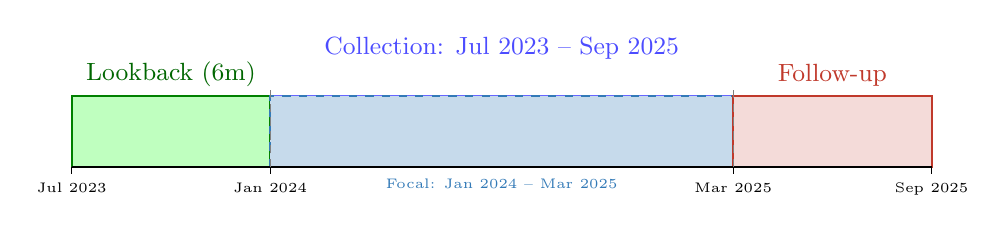
\begin{tikzpicture}[x=0.42cm,y=1cm]

% --- Main collection window ---
\fill[blue!8] (0,0) rectangle (26,0.9);
\draw[blue!60, thick] (0,0) rectangle (26,0.9);

% --- Lookback ---
\fill[green!25] (0,0) rectangle (6,0.9);
\draw[green!50!black, thick] (0,0) rectangle (6,0.9);

% --- Focal ---
\fill[accentblue!28] (6,0) rectangle (20,0.9);
\draw[accentblue, thick, dashed] (6,0) rectangle (20,0.9);

% --- Follow-up ---
\fill[alertred!18] (20,0) rectangle (26,0.9);
\draw[alertred, thick] (20,0) rectangle (26,0.9);

% Labels
\node[green!40!black, above] at (3,0.9) {\small Lookback (6m)};
\node[accentblue, below] at (13,-0.02) {\tiny Focal: Jan 2024 -- Mar 2025};
\node[alertred, above] at (23,0.9) {\small Follow-up};

\node[blue!70, above] at (13,1.25) {\small Collection: Jul 2023 -- Sep 2025};

% Axis
\draw[thick] (0,0) -- (26,0);
\foreach \x/\lbl in {
  0/{Jul 2023},
  6/{Jan 2024},
  20/{Mar 2025},
  26/{Sep 2025}
}{
  \draw (\x,0) -- (\x,-0.08);
  \node[below] at (\x,-0.08) {\tiny \lbl};
}

\draw[densely dashed, gray] (6,0) -- (6,1.05);
\draw[densely dashed, gray] (20,0) -- (20,1.05);

\end{tikzpicture}
\end{center}

\vspace{0.5em}

\begin{itemize}
  \item \textbf{Focal PRs}: Jan 2024 -- Mar 2025 (analysis set)
  \item \textbf{Lookback}: classify newcomers
  \item \textbf{Follow-up}: measure return
\end{itemize}

\begin{alertblock}{Why this design}
Avoids \textbf{mislabeling experience} and \textbf{incomplete return data}
\end{alertblock}

\end{frame}

\begin{frame}{Part 3\\Methods and Pipeline}

\begin{block}{Data collection}
GitHub REST API:
\begin{itemize}
  \item PR metadata
  \item issue comments
  \item review comments
\end{itemize}
\end{block}

\vspace{0.4em}
\begin{block}{NLP signals}
\begin{itemize}
  \item toxicity (max + thresholds)
  \item sentiment
  \item anger
  \item politeness
\end{itemize}
\end{block}

\vspace{0.4em}
\begin{exampleblock}{Pipeline}
collect $\rightarrow$ comments $\rightarrow$ dataset $\rightarrow$ NLP $\rightarrow$ analysis
\end{exampleblock}

\end{frame}

\begin{frame}{Part 3\\Challenges}

\begin{itemize}
  \item Toxicity likely sparse
  \item Technical language may confuse NLP
  \item Experience may dominate outcomes
  \item Observational study (no causality)
  \item PR-only return misses other activity
\end{itemize}

\vspace{0.6em}
\begin{alertblock}{Expectation}
Communication tone may still matter through
\textbf{sentiment, politeness, and interaction structure}
\end{alertblock}

\end{frame}



% ────────────────────────────────────────────────────────────────
\begin{frame}
\vfill
\begin{center}
{\Huge\bfseries Thank you}
\end{center}
\vfill
\end{frame}

\end{document}